\lfoot{Autor: Hüseyin Bozkurt}
\subsection{Umweltbelastung durch \ce{CO2} Ausstoß}


\textbf{Was ist CO_{2}?}
CO_{2} wird umgangssprachlich Kohlenstoffdioxid genannt und ist die zusammengesetzt aus einem Kohlenstoff-Atom und zwei Sauerstoff-Atomen. 
Die charkteristischen Eigenschaften von CO_{2} sind Unsichtbarkeit und Geruchslosigkeit. 
In jedem Stoffwechselprozess spielt Kohlenstoffdioxid eine wichtige Rolle, da beispielsweise der Mensch CO_{2} ausatmet. 
Bei vielen Energiegewinnungsverfahren werden durch Verbrennung Energien freigesetzt, die als Nebenprodukt Kohlenstoff produzieren. 
In der freien Luft werden diese Kohlenstoffpartikel zu CO_{2}.
CO_{2} ist Reaktionsträge und besitzt keine giftige Eigenschaft. 
Das Problem mit den Unmengen an ausgestoßenem CO_{2} ist, dass sein massives Vorkommen die Atmosphäre beschädigt.

\textbf{Wie entsteht CO_{2}?}
Alle Fahrzeuge, die Kraftstoffe als Energiequelle nutzen 
(wie zum Beispiel Diesel, Flüssiggas, Benzin und auch Biotreibstoff), erzeugen Kohlenstoff als Abgas. 
Indem der Motor den Kraftstoff zusammen mit Luftsauerstoff verbrennt, gelangt das CO_{2} über die Abgasanlage in die Atmosphäre. 
Eine effektive Methode zur Beseitigung der Kohlenstoffpartikel gibt es zurzeit nicht. 
Der benutzte Kraftstoff bestimmt, wie viel CO_{2} bei der Verbrennung als Nebenprodukt entsteht.
Beispielsweise entsteht bei der Verbrennung von einem Liter Diesel mehr Kohlenstoffdioxid, als bei einem Liter Benzin.
Der Kraftstoffverbrauch eines Kraftfahrzeugs und sein CO_{2}-Output stehen daher in enger Verbindung.
Demnach existieren Werte, die man als Grenze für den Verbrauch festlegen kann. 
Heutzutage spricht man von der Einheit Gramm pro Kilometer [g/km] als normierte Verbrauchsmessung.
Der Lenker eines PKW hat natürlicherweise Einfluss auf seinen CO_{2}-Ausstoß. 
Dieses Umweltbewusstsein wollen wir im Rahmen dieser Diplomarbeit weitervererben, indem wir den Benutzerinnen und Benutzern 
von BestShift Tipps zum sparsamen und umweltschonenden Fahren geben.

\textbf{Ökologische Hintergründe (Treibhauseffekt)}
Kohlenstoffdioxid ist ein sogenanntes Abfallprodukt, welches bei Verbrennungsprozessen zur Energiegewinnung entsteht. 
CO_{2} gilt als Vorreiter der Treibhausgase.
Die negative Umweltauswirkung, welche zustande kommt indem Unmengen an CO_{2} in die Atmosphäre gelangen, 
nennt sich Treibhauseffekt. 
Der Treibhauseffekt ist eine der Hauptursachen für den Klimawandel, welcher drastische Folgen für Natur, Tiere und Menschen hat. 
Zu viel CO_{2} in der Atmosphäre bringt unter anderem das Abschmelzen von Gletschern, 
den Anstieg der Meerestemperatur, den Anstieg des Meeresspiegels, 
Aussterben von Pflanzen und Tieren und Wetterphänomene wie zum Beispiel sehr warme Winter, Stürme etc.
Das Kohlenstoffdioxid steigt bis zur Atmosphäre auf und bildet dort eine "Mauer".
Sonnenstrahlen können zwar ohne weiteres durch, doch nicht so leicht wieder raus. Das heisst, dass die Sonnenstrahlen,
die von der Erdoberfläche wieder zurück in den Weltraum reflektiert werden sollten, von der Erdatmosphäre zurück auf die Erde geworfen werden. 

\begin{figure}[!htb]\centering
	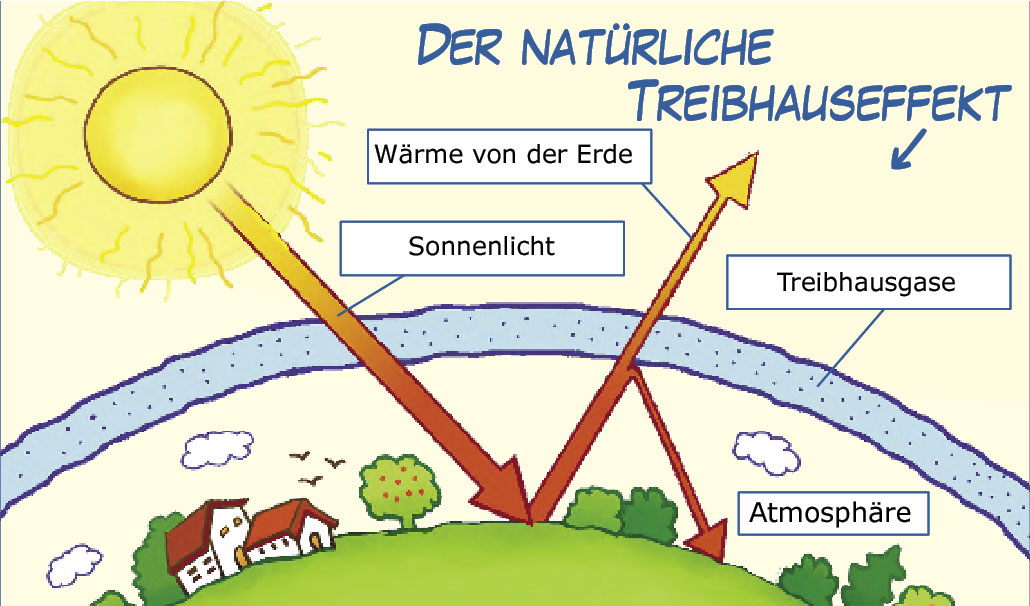
\includegraphics[width=0.5\textwidth]{images/treibhaus1}
	\caption{Der Treibhauseffekt \cite{BOZH.ch1-co2-umwelt.treibhaus1}}\label{Fig:Data3}
\end{figure}
 
\textbf{Das Kyoto-Protokoll}
Im Rahmen des Kyoto-Protokolls haben sich viele westliche Staaten zu einer Reduktion der Treibhausgase verpflichtet. 
Dieses Protokoll war der Startschuss für die Suche nach erneuerbaren Energien. 
Anfang 2015 sind Gesetzesregelungen in Kraft getreten, die den Durchschnittsverbrauch eines PKW auf 130g/CO_{2} pro kilometer limitierten. 
Bis 2020 soll dieses Limit auf 95g/CO2 pro kilometer herunter gesetzt werden.

\textbf{Definition und Enstehung\nextline}
Kohlenstoffdioxid ist die zusammmensetzung aus einem Kohlenstoff-Atom und zwei Sauerstoff-Atomen. Die charkteristischen Eigenschaften von \ce{CO2} sind Unsichtbarkeit und Geruchslosigkeit. In jedem Stoffwechselprozess spielt Kohlenstoffdioxid eine wichtige Rolle; beispielsweise atmet der Mensch das Dioxid aus. Bei vielen Energiegewinnungsverfahren werden durch Verbrennung Energien freigesetzt, die als Nebenprodukt Kohlenstoff produzieren. In der freien Luft werden diese Kohlenstoffpartikel zu \ce{CO2}, wobei das Dioxid nur ein Reaktionsträger ist und an sich keine giftige Eigenschaft besitzt. Das Problem mit den Unmengen an ausgestoßenem Schadstoffen ist, dass sein massives Vorkommen die Atmosphäre beschädigt.

Alle Fahrzeuge, die Kraftstoffe als Energiequelle nutzen, wie zum Beispiel Diesel, Flüssiggas, Benzin und auch Biotreibstoff, erzeugen Kohlenstoff als Abgas. Indem der Motor den Kraftstoff zusammen mit Luftsauerstoff verbrennt, gelangt das \ce{CO2} über die Abgasanlage in die Atmosphäre. Eine effektive Methode zur beseitigung der Kohlenstoffpartikel gibt es zurzeit nicht. Der benutzte Kraftstoff bestimmt, wie viel \ce{CO2} bei der Verbrennung erzeugt wird. Beispielsweise entsteht bei der Verbrennung von einem Liter Diesel mehr Kohlenstoffdioxid, als bei einem Liter Benzin.Der Kraftstoffverbrauch eines Wagens und sein \ce{CO2}-Output stehen daher in enger Verbindung. Demnach existieren Werte, die man als Grenze für den Verbrauch festlegen kann. Heutzutage spricht man von der Einheit gramm pro kilometer als normierte Verbrauchsmessung.Der Lenker eines PKW hat natürlicherweise Einfluss auf seinen \ce{CO2}-Ausstoß. Dieses Umweltbewusstsein wollen wir im Rahmen dieser Diplomarbeit weitervererben, indem wir den Benutzerinnen und Benutzern von BestShift Tipps zum sparsamen und umweltschonenden Fahren geben.

\textbf{Das Kyoto-Protokoll\nextline}
Im Rahmen des Kyoto-Protokolls haben sich viele westliche Staaten zu einer Reduktion der Treibhausgase verpflichtet. 
Dieses Protokoll war der Startschuss für die Suche nach erneuerbaren Energien. 
Anfang 2015 sind Gesetzesregelungen in Kraft getreten, die den Durchschnittsverbrauch eines PKW auf 130g/\ce{CO2} pro kilometer limitierten. 
Bis 2020 soll dieses Limit auf 95g/\ce{CO2} pro Kilometer herunter gesetzt werden.




\clearpage % DO NOT REMOVE